\section{Threshold Analysis}\label{sec:threshold_analysis}

In the previous sections, we have described two separate voting phases in the 
decentralized software update lifecycle (figure \ref{lifecycle}), namely 
Ideation and Approval, where a proposal can be approved or rejected by the 
community. Moreover, during the Activation phase the community, or more 
accurately, the participants in the blockchain consensus protocol, signal 
\emph{upgrade readiness} by endorsing a new version of the protocol. Both of 
these processes are based on a \emph{threshold} of stake percent, against 
which, 
the gathered votes/signals are compared. Although the voting of a proposal 
compared to the activation of a proposal have different end-goals, there 
are still a lot of commons from a social dynamics perspective. In this section, 
we present an analysis towards a unified approach for defining an appropriate 
threshold for both of these two processes.

Lets assume that $H$ is the percent of honest stake and $T$ is the percent of 
adversarial stake that actively participate in the voting (or activation) 
process. We assume 
also that
\begin{equation}\label{eq:H_plus_T}
	H+T=100    
\end{equation}
%Moreover, the stake considered during the tally is the stake that the voters 
%have at that moment. That is, we only consider the stake of the voters at the 
%moment of the tally, without taking into account the stake that the voters had 
%in the moment that the votes were casted. In other words, the calculation of 
%the voting result corresponds to the stake distribution at the same time and 
%not to some previous historic moment. This way, the result better represents 
%the current situation at the moment of the tally.

We consider two types of possible attacks relevant to both processes:
\paragraph{Voting process}
\begin{itemize}
	\item \textbf{Malicious Proposal Attack}: The 
	adversary manages with its own stake to approve a malicious proposal.
	\item \textbf{Denial of Approval Attack}: The adversary manages to block a 
	good 
	proposal approved by the honest stake.
\end{itemize}

\paragraph{Activation process}
\begin{itemize}
	\item \textbf{Rushing Adversary Attack}: The adversary rushes, by using its 
	own stake, to signal upgrade readiness and cause the activation of the 
	changes, in order to take over the control of the updated blockchain, 
	before enough honest parties manage to upgrade. 
	\item \textbf{Denial of Activation Attack}: The 
	adversary manages to block the activation of a change signaled by the 
	honest stake.
\end{itemize}


With respect to the two said attacks for each process, we define next, the 
notion of a secure voting (or activation) protocol:
\begin{definition}\label{def:liveness_safety_voting}
	A voting protocol is secure, if it enjoys both the safety 
	and liveness properties.
	
	\begin{itemize}
		\item \textbf{Safety property for voting:} a software update that has 
		achieved 
		only the adversary stake approval, will never be approved.
		
		\item \textbf{Liveness property for voting:} a software update that has 
		achieved 
		sufficient honest stake $L_b$ approval, will be eventually approved, 
		i.e., cannot be blocked by the adversary stake.		
	\end{itemize}	
\end{definition}


\begin{definition}\label{def:liveness_safety_activation}
	An activation protocol is secure, if it enjoys both the safety 
	and liveness properties.
	
	\begin{itemize}
		\item \textbf{Safety property for activation:} a software update that 
		has not received signals of sufficient  stake w.r.t. the 
		security assumption of the upgraded protocol (see section 
		\ref{secureupdate}), will never be activated.
		
		\item \textbf{Liveness property for activation:} a software update that 
		has received
		signals of sufficient honest stake $L_b$, will be eventually activated, 
		i.e., cannot be blocked by the adversary stake.		
	\end{itemize}	
\end{definition}

Clearly, the safety property protects us from the malicious approval/rushing 
adversary attack, 
while the liveness property protects us from the denial of approval/activation 
attack.

Our goal, is to define an appropriate voting/adoption threshold $\tau$, such 
as the two said properties hold. 
\begin{definition}
	A voting threshold $\tau_V$ (see section \ref{appxvoting}) is an amount of 
	stake such that any stake $p 
	> \tau_V$ of positive votes can approve a proposal and any stake $n > 
	\tau_V$ of 	negative votes can reject a proposal.
\end{definition}
Similarly,
\begin{definition}
	An adoption threshold $\tau_A$ (see section \ref{secureupdate}) is 
	an amount of stake such that any stake $p 
	> \tau_A$ of signals can activate a proposal.
\end{definition}

%In our analysis, we will need two boundary 
%values: 
%\begin{inparaenum}[\itshape a)\upshape]
%	\item a minimum of honest stake that should control the result and
%	\item a maximum of adversary stake that should not be able to control the 
%	result.
%\end{inparaenum} We define them both next.
%
%\begin{definition}\label{def:liveness-bound}
%	We define as \emph{liveness bound} $L_b$ the minimum percent of  
%	stake that our voting (or activation) protocol allows to control the 
%	result, 
%	i.e., the minimum amount of stake required for a result not to be 
%	blocked.
%\end{definition}
%
%\begin{definition}\label{def:safety-bound}
%	We define as \emph{safety bound} $S_b$ the maximum percent of 
%	stake that our voting (or activation) protocol prevents from controlling 
%	the 
%	result.
%\end{definition}
%
%Intuitively, we would like $L_b$ to correspond to some amount of the honest 
%stake, i.e., $0 \leq L_b \leq H$ that we wish not to be blocked when voting 
%for 
%(or signaling for) 
%a proposal and $S_b$ to correspond to some amount of the 
%adversary stake, i.e., $0 \leq S_b \leq T$ that we want to prevent from 
%approving (or activating) a proposal. The following theorem defines the 
%necessary and 
%sufficient condition that the threshold $\tau$ should satisfy, in order both 
%the safety and liveness properties to hold.

Next we define the sufficient and necessary condition for the voting threshold 
and the adoption threshold in order for safety and liveness to hold
\begin{theorem}\label{th:safety_and_liveness_condition_voting}
	For each voting protocol with a threshold $\tau_V$ 
	both the safety and liveness properties hold iff:
	\begin{align*} 
		T < \tau_V < H 
	\end{align*}
	\begin{proof}
		Since $T < \tau$, any malicious proposal that is voted positively by 
		the adversarial stake $T$, but by no honest stake at all, cannot be 
		approved, because the condition for approval is $[positive\ stake] > 
		\tau$. Therefore, the safety property holds. Inversely, if the safety 
		property holds, then no proposal that has no positive votes from the 
		honest stake can be approved even if the adversary stake $T$ has 
		voted in favor, which means that the positive votes must be below the 
		voting threshold; thus $T < \tau$. 
		
		Similarly, since $\tau < H$, any proposal that has 
		received $L_b$, or more, positive votes from the honest stake, where $ 
		\tau_V < L_b \leq H$ will be 
		approved, because the condition for approval is $[positive\ stake] > 
		\tau$. Inversely, if the liveness condition holds, then any proposal 
		that has received at least $L_b$ positive votes from the honest stake 
		will be approved, which means that the following 
		condition should hold $\tau < L_b$.
	\end{proof}
\end{theorem}

The adoption threshold $\tau_A$ should ensure that the required percent of 
stake that has signaled upgrade readiness, will guarantee that 
the new blockchain will kick off with sufficient honest stake, determined by 
the 
security assumption of the upgraded consensus protocol. It is easy to 
see that in this case, we need $\tau_A \geq \frac{1}{r_{Th}} \times T$, where 
$r_{Th}$ corresponds to the theoretical adversary tolerance of the 
\emph{upgraded protocol} (potentailly different from the original protocol),  
so that for the upgraded stake, the required security property
$\frac{AdversaryStake}{TotalStake_{upgraded}} < r_{Th}$ will still hold and 
thus the upgraded blockchain will be secure. Indeed, if we assume that the 
total upgraded stake percent is above the adoption threshold minimum value 
$\frac{1}{r_{Th}} \times T$ (e.g., $\frac{1}{r_{Th}} \times T + \delta$ where 
$\delta > 0$) and that all the adversary stake $T$ has upgraded (so we have $T$ 
percent of adversaries in the new blockchain too), then if we 
substitute, we see that the property 
$\frac{AdversaryStake}{TotalStake_{upgraded}} = \frac{T}{\frac{1}{r_{Th}} 
\times T + \delta} < r_{Th}$ holds for the upgraded protocol. So 
$\frac{1}{r_{Th}} T$ is the appropriate lower bound for the adoption threshold, 
in order to ensure safety. Here is the respective theorem for the adoption 
threshold.

\begin{theorem}\label{th:safety_and_liveness_condition_activation}
	For each activation protocol with a threshold $\tau_A$ 
	both the safety and liveness properties hold iff:
	\begin{align*} 
		\frac{1}{r_{Th}}T < \tau_A < H 
	\end{align*}
	where $r_{Th}$ is the 
	theoretical 
	adversary tolerance of our consensus protocol.
	\begin{proof}
		Since $\frac{1}{r_{Th}}T < \tau$, signals of any stake not sufficient 
		w.r.t. the security assumption of the upgraded protocol (see section 
		\ref{secureupdate}), cannot cause the activation of the changes, 
		because the condition for activation is $[signals'\ stake] > 
		\tau_A$. Therefore, the safety property holds. Inversely, if the safety 
		property holds, then any proposal that has not sufficient stake 
		signaled cannot be activated, which means that $\frac{1}{r_{Th}}T < 
		\tau$. 
		
		Similarly, since $\tau < H$, any proposal that has 
		received signals of stake $L_b$ or more, from the honest stake, where $ 
		\tau_A < L_b \leq H$ will be 
		activated, because the condition for approval is $[signals'\ stake] > 
		\tau_A$. Inversely, if the liveness condition holds, then any proposal 
		that has received signals of stake  at least $L_b$ from the honest 
		stake 
		will be activated, which means that the following 
		condition should hold $\tau_A < L_b$.
	\end{proof}
\end{theorem}
%\begin{theorem}\label{th:safety_and_liveness_condition}
%	For each voting (or activation) protocol with a voting threshold $\tau_V$ 
%	both the safety 
%	and liveness properties hold iff:
%	\begin{align*} 
%		T < \tau_V < \frac{H}{2} + \mu,\ where\ 0 < \mu \leq \frac{H}{2}
%		% &T < \tau_V < \frac{H}{2} + \mu\ \ \ \ \land\\ 
%		% &T < \frac{H}{2} \overset{eq. \ref{eq:H_plus_T}}{\iff} T < 
%		%\frac{1}{3} \times 100,\\  
%		% &where\ 0 < \mu \leq \frac{H}{2}
%	\end{align*}
%	\begin{proof}
%		Since $T < \tau_V$, any malicious proposal that is voted positively by 
%		all adversarial stake T, but by no honest stake at all, cannot be 
%		approved, because the condition for approval is $[positive\ stake] > 
%		\tau_V$. Therefore, the safety property holds. Inversely, if the safety 
%		property holds, then no proposal that has no positive votes from the 
%		honest stake can be approved even if the whole adversary stake has 
%		voted in favor, which means that the positive votes must be below the 
%		voting threshold; thus $T < \tau_V$. 
%		
%		Similarly, since $\tau_V < \frac{H}{2} + \mu$, any proposal that has 
%		received $\frac{H}{2}+\mu$ positive votes, where $0 < \mu \leq 
%		\frac{H}{2}$ from the honest stake will be approved, because the 
%		condition for approval is $[positive\ stake] > \tau_V$. Inversely, if 
%		the liveness condition holds, then any proposal that has received 
%		$\frac{H}{2}+\mu$ positive votes, where $0 < \mu \leq \frac{H}{2}$ from 
%		the honest stake will be approved, which means that the following 
%		condition should hold $\tau_V < \frac{H}{2} + \mu$.
%	\end{proof}
%\end{theorem}

In the following, we propose a threshold function $\tau(\gamma)$, which depends 
on a 
parameter $\gamma$ that we call the \emph{safety strength} and adjusts the 
threshold towards liveness or safety. We provide also the 
sufficient conditions, in order for both safety and liveness properties to 
hold. Intuitively,   if we increase the threshold, we increase the required 
amount of honest-stake positive votes required (or signals), in order to 
approve (or activate) a proposal. This means that we decrease liveness, but at 
the same time we increase safety, since it becomes more difficult for a 
malicious proposal to be approved (or for activation without a sufficient 
amount of stake to take place). The definition of the threshold function 
includes also 
a fixed amount of honest stake $H_{min}$, which is the minimum value that we 
want our threshold to have and essentially determines the minimum amount of 
honest stake that we wish not to be blocked (either for voting or activation), 
i.e., it determines the minimum amount of honest stake that we wish the 
liveness property to hold.

Although the threshold function definition is common for both voting and 
activation, since they differ on the required constraint, we present them in 
two separate theorems:
\begin{theorem}\label{th:proposed_voting_threshold}
	If the threshold $\tau$ of a voting protocol is 
	defined as:
	\begin{align*}
		&\tau(\gamma) = H_{min} + \gamma,\ where\ 0 \leq \gamma < H-H_{min} \\
		&\land\\
		&T < H_{min}\\
	\end{align*}
,where  $0 \leq H_{min} \leq H$,
then both the safety and liveness properties hold for any amount of honest 
stake $L_b$ such that $H_{min} + \gamma < L_b \leq H$.
	\begin{proof}
		Since 
		\begin{align*}
			&T < H_{min} \iff\\
			&T < H_{min} + \gamma \iff\\
			&T < \tau(\gamma)
		\end{align*}
		Also, since $H_{min} + \gamma < L_b \leq H$, then we have $\tau(\gamma) 
		< H$.
		Therefore we have proved that $T < \tau(\gamma) < H$ and thus 
		based on theorem \ref{th:safety_and_liveness_condition_voting} both 
		safety 
		and 
		liveness properties hold.
	\end{proof}
\end{theorem}

\begin{theorem}\label{th:proposed_adoption_threshold}
	If the threshold $\tau$ of an activation protocol is 
	defined as:
	\begin{align*}
		&\tau(\gamma) = H_{min} + \gamma,\ where\ 0 \leq \gamma < H-H_{min} \\
		&\land\\
		&\frac{1}{r_{Th}}T < H_{min}\\
	\end{align*}
	,where $0 \leq H_{min} \leq H$,
	then both the safety and liveness properties hold for any amount of honest 
	stake $L_b$ such that $H_{min} + \gamma < L_b \leq H$.
	\begin{proof}
		Since 
		\begin{align*}
			&\frac{1}{r_{Th}}T < H_{min} \iff\\
			&\frac{1}{r_{Th}}T < H_{min} + \gamma \iff\\
			&\frac{1}{r_{Th}}T < \tau(\gamma)
		\end{align*}
		Also, since $H_{min} + \gamma < L_b \leq H$, then we have $\tau(\gamma) 
		< H$.
		Therefore we have proved that $\frac{1}{r_{Th}}T < \tau(\gamma) < H$ 
		and thus 
		based on theorem \ref{th:safety_and_liveness_condition_activation} both 
		safety 
		and 
		liveness properties hold.
	\end{proof}
\end{theorem}


%From section \ref{secureupdate}, we have seen that the appropriate choice for 
%$S_b$ during the activation phase is $S_b = \frac{1}{r_{Th}}\times T$. This is 
%in order to ensure that the amount of stake that has signaled upgrade 
%readiness 
%guarantees that the security assumption of the updated protocol will hold and 
%that the adversary cannot take over of the updated blockchain. In addition, 
%for 
%a voting process the appropriate choice for $S_b$ is $S_b = T$, in order to 
%ensure that the malicious approval attack cannot take place.
%
%The $H_{min}$ can take any value in the range $0 \leq H_{min} \leq H$, as long 
%as 
%the condition $S_b < H_{min}$ holds. The $H_{min}$ corresponds to the lowest 
%value 
%that we are willing to give to the liveness bound $L_b$. Therefore, it is the 
%minimum of honest stake that we wish to be able to approve a result. A typical 
%value for 
%$H_{min}$ could 
%be $H_{min} = \frac{H}{2}$, which means that we require that any result 
%approved by the honest stake majority should not be blocked. In this case, and 
%for 
%$S_b = T$, the condition $S_b < H_{min}$ becomes $T < \frac{H}{2}$, which 
%translates to $r < 1/3$, where $r$ is the adversary ratio. 

The $\gamma$ parameter (safety strength) allows us to adjust the threshold 
towards liveness, or 
safety. This is depicted in figure \ref{fig:gamma_parameter}. Low gamma values 
provide thresholds with a greater liveness, but reduced safety and inversely, 
high $\gamma$ values enable higher safety, but less liveness. This applies to 
both the voting and the activation processes and this figure corresponds to 
both.

\begin{figure}[h!] %[H]
	\centering
	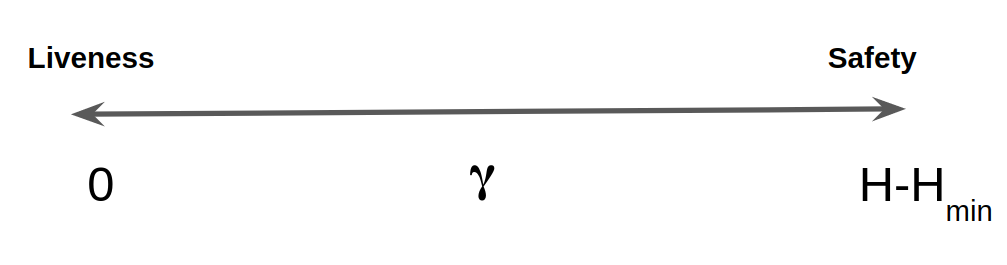
\includegraphics[width=0.6\columnwidth,
	keepaspectratio]{figures/gamma.png}
	\caption{The $\gamma$ parameter versus liveness and safety for either 
	voting or activation.}
	\label{fig:gamma_parameter}
\end{figure}

This parametric definition of the threshold gives us the ability to adjust the 
threshold based on the context of each individual proposal and not follow a one 
size fits all approach. For example, for a very critical update we might 
require a higher $\gamma$ value in order to ensure a greater safety for the 
result by sacrificing some of the liveness and demanding a stronger consent 
from the community. 

Table \ref{table:threshold_examples} shows some examples of different 
threshold functions $\tau(\gamma)$, expressed by means of 
the adversary stake ratio $r$, $r = \frac{Adversary\ Stake}{Total\ Stake} = 
\frac{T}{T+H} = \frac{T}{100}$, along with the corresponding constraint on $r$, 
derived from the $T < H_{min}$ constraint and $\frac{1}{r_{Th}}T < H_{min}$ 
constraint for voting and activation respectively. The choice of $H_{min}$ 
recorded on the second column determines the resulting threshold function, as 
well as the required constraint, appearing in the respective columns. Our 
analysis is based on the assumption 
that we can have an estimation of the adversary ratio $r$. From Garay et. al. 
in \cite{sok}, we know that the 
ratio $r$ is always upper bounded by the 
theoretical 
adversary tolerance $r_{Th}$ of our consensus protocol, i.e., $r < r_{Th}$ 
(e.g., $r < 1/2 = 
r_{Th}$, or $r < 1/3 = r_{Th}$ etc.).

\begin{table}[h!]
	\centering
	\begin{tabular}{ | c | c | c | c |} 
		\hline
		\textbf{Process} & $H_{min}$ & \makecell[c]{\textbf{Threshold}\\ 
		$\tau(\gamma) = 
		H_{min} + \gamma$,\\ where $0 \leq \gamma < H-H_{min}$} & 
		\makecell[c]{\textbf{Constraint}\\$T < H_{min}$ (for voting)\\ 
		$\frac{1}{r_{Th}T} < H_{min}$ 
		(for activation)} \\ 
		\hline
		\multirow{2}{*}{Voting} & $\frac{H}{2}$ & 
		$50(1-r)+\gamma$ & $r < 1/3$
		 \\ 
		 & $T+1$ & $100r + 1 +\gamma$ & Any $r < r_{Th}$ \\ 
		\hline
		\multirow{2}{*}{Activation} & $\frac{H}{2}$ & 
		$50(1-r)+\gamma$ & 
		\makecell[c]{$r < \frac{r_{Th}}{2+r_{Th}}$ \\ ($r < 1/5$ for 
		$r_{Th} = 1/2$)}
		\\ 
		 & $\frac{1}{r_{Th}}T + 1$ & 
		$\frac{100r}{r_{Th}} + 1 + \gamma$ & Any $r < r_{Th}$ \\ 
		\hline
	\end{tabular}
	\caption{Examples of different threshold definitions.}
	\label{table:threshold_examples}
\end{table}

In table \ref{table:examples}, we provide examples of threshold 
values for different values of $\gamma$ and different adversary ratios r for a 
specific choice of the $\tau(\gamma)$ function and a constraint relevant to the 
voting process. In particular, for the function $\tau(\gamma) = H/2 + \gamma = 
50(1-r)+\gamma$ and $r < 1/3$ (i.e., $H_{min} = 
\frac{H}{2}$ and $T < \frac{H}{2}$). For a specific adversary ratio r, as we 
increase $\gamma$, we 
require stronger honest stake majority, in order to avoid the denial of 
approval attack, however this provides us with more safety. In this particular 
case of $\tau(\gamma)$, the 
allowed $\gamma$ values lie in the range $0 \leq \gamma < H/2$.  So in the 
table 
we have chosen the lowest possible $\gamma$ value ($\gamma=0$), the maximum 
$\gamma$ value ($\gamma = \frac{H}{2} - 1$) (assuming for the sake of the 
example that $\gamma$ takes integer values) and an intermediate value $\gamma = 
T$.

So for instance, in the line where $r=0.1$, we can see that the allowed range 
of values for the threshold is $[45\%, 89\%]$. As long as the threshold is 
in this range, we can have both liveness and safety (assuming $r=0.1$).We 
observe that for low values of $\gamma$ ($\gamma = 0$), $H/2$ of honest stake 
is 
enough to have liveness. In contrast, for high values of $\gamma$ ($\gamma = 
H/2 -1$), we essentially require honest stake unanimity in order to have 
liveness.
%Looking 
%at the columns we can see that the voting threshold gradually decreases when r 
%increases for a fixed value of $\gamma = 0$. While this is not the case in the 
%$\gamma = T$ column, where the threshold increases since it is linearly 
%depended on T ($\tau = 50 + \frac{T}{2}$). Finally, in the last column, the 
%threshold decreases because it is linearly depended on H ($\tau = H - 1$) and 
%H decreases as r increases.

\begin{table}[h!]
	\centering
	\begin{tabular}{ | c | c | c | c |} 
		\hline
		Adversary ratio r ($r < 1/3 \approx 0.33$) & $\gamma = 0$ & $\gamma = 
		T$ & $\gamma = \frac{H}{2} - 1$ \\ 
		\hline
		$0.1$ & $45\%$ & $55\%$ & $89\%$ \\ 
		$0.2$ & $40\%$ & $60\%$ & $79\%$ \\ 
		$0.3$ & $35\%$ & $65\%$ & $69\%$ \\ 
		\hline
	\end{tabular}
	\caption{Threshold values for different $\gamma$ and adversary 
		ratios for a specific choice of $\tau(\gamma)$ ($\tau(\gamma) = 
		50(1-r)+\gamma$), relevant to the voting 
		process.}
	\label{table:examples}
\end{table}

%Theorem \ref{th:proposed_voting_threshold} provides a definition of the voting 
%threshold that is sufficient for both the safety and liveness properties to 
%hold. This holds only when the adversary stake $T < 1/3 \times 100 \approx 
%33.33\%$. The $\gamma$ parameter can essentially take values in the range $0 
%\leq \gamma < \frac{H}{2}$ and is always upper bounded by the strength of the 
%honest majority result $\mu$. This means that \emph{only} honest majority 
%results of strength $\mu > \gamma$ cannot be blocked (i.e., the liveness 
%property holds).
%
%For $\gamma = 0$, $\tau_V = \frac{H}{2}$, which means that an honest majority 
%result of \emph{any} strength $\mu$ will be approved (i.e., cannot be 
%blocked), 
%even if the honest majority is marginal, i.e., just $\frac{H}{2} + 1$. On the 
%other hand, such a low threshold $\tau_V$, increases the risk of violating the 
%safety property, since in the case of a malicious proposal voted in favor by 
%the adversary stake T, there are only $\frac{H}{2} - T + 1$ positive votes 
%missing for the proposal to be approved. So we could say informally that when 
%$\gamma$ values are low, liveness is positively impacted, while safety is 
%negatively impacted. Inversely, when $\gamma$ is close to $\frac{H}{2}$, then 
%$\tau_V$ increases and becomes very difficult to violate safety. However, we 
%know that only stake majority results of strength $\mu>\gamma$ cannot be 
%blocked and since $\gamma$ is high valued, the set of results that cannot be 
%blocked reduces. So we could say informally that when $\gamma$ values are 
%high, 
%liveness is negatively impacted, while safety is positively impacted. The 
%relation of the $\gamma$ parameter to the safety and liveness properties is 
%depicted in figure \ref{fig:gamma_parameter}.
%
%\begin{figure}[h!] %[H]
%	\centering
%	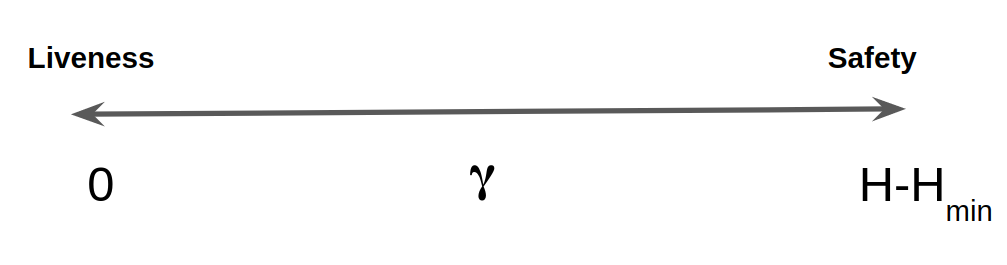
\includegraphics[width=0.6\columnwidth,
%	keepaspectratio]{figures/gamma.png}
%	\caption{The $\gamma$ parameter versus liveness and safety.}
%	\label{fig:gamma_parameter}
%\end{figure}
%
%We see from theorem \ref{th:proposed_voting_threshold} that the proposed 
%voting 
%threshold is lower bounded by $\frac{H}{2}$. It can be easily proved that it 
%could be lower bounded even by $T$, where $T < \frac{H}{2}$. In other words, 
%we 
%could have chosen $\tau_V(\gamma) = T + \gamma$ where $0 < \gamma < \mu$ and 
%still enjoy the properties of safety and liveness. We have chosen to lower 
%bound $\tau_V$ by $\frac{H}{2}$, because we want to honor honest stake 
%\emph{majority} and not \emph{minority}. For example, if $T=20\%$ ($H=80\%$) 
%and we have 
%chosen 
%$\tau_V = 25\%$, then even a $30\%$ of honest stake positive votes would be 
%enough to approve a result, assuming that the rest $50\%$ of 
%the honest stake does not vote, or that their votes are split to $25\%$ reject 
%and $25\%$ abstain votes. Since we do not want to allow honest minority to 
%control the voting result like this we have decided to lower bound $\tau_V$ by 
%$\frac{H}{2}$.
%
%Another important observation is that our analysis is based on the assumption 
%that we can have an estimation of the adversary ratio $r$. If it is not 
%possible to estimate $r$ with some accuracy, then we could take a worst case 
%approach for estimating $r$. From Garay et. al. in \cite{sok}, we know that 
%the 
%ratio $r = \frac{T}{T+H} = \frac{T}{100}$ is always upper bounded by the 
%theoretical 
%adversary tolerance $r_{Th}$ of our consensus protocol, i.e., $r = 
%\frac{AdversaryStake}{TotalStake} = \frac{T}{100} < r_{Th}$ (e.g., $r < 1/2 = 
%r_{Th}$, or $r < 1/3 = r_{Th}$ etc.).
%
%In table \ref{table:examples}, we provide some examples of the voting 
%threshold 
%$\tau_V$ for different values of $\gamma$ and different adversary ratios r.For 
%a specific adversary ratio r, as we increase $\gamma$, we require stronger 
%honest stake majority, in order to avoid the denial of approval attack. 
%Looking 
%at the columns we can see that the voting threshold gradually decreases when r 
%increases for a fixed value of $\gamma = 0$. While this is not the case in the 
%$\gamma = T$ column, where the threshold increases since it is linearly 
%depended on T ($\tau_V = 50 + \frac{T}{2}$). Finally, in the last column, the 
%threshold decreases because it is linearly depended on H ($\tau_V = H - 1$) 
%and 
%H decreases as r increases.
%
%\begin{table}[h!]
%	\centering
%	\begin{tabular}{ | c | c | c | c |} 
%		\hline
%		Adversary ratio r ($r < 1/3 \approx 0.33$) & $\gamma = 0$ & $\gamma = 
%		T$ & $\gamma = \frac{H}{2} - 1$ \\ 
%		\hline
%		$0.1$ & $45\%$ & $55\%$ & $89\%$ \\ 
%		$0.2$ & $40\%$ & $60\%$ & $79\%$ \\ 
%		$0.3$ & $35\%$ & $65\%$ & $69\%$ \\ 
%		\hline
%	\end{tabular}
%	\caption{Voting threshold values for different $\gamma$ and adversary 
%		ratios.}
%	\label{table:examples}
%\end{table}
